\section{Selection}
\label{sec:kstmm:sel}

The aim of the \BdToKstmm event selection is to select complete \BdToKstmm candidates from the triggered data. 
As mentioned in Section~\ref{sec:lhcb:trigdev}, biases in the selection of \BdToKstmm candidates have the effect of removing events which contribute 
the most to measurements of \AFB. The trigger lines, the pre-selection  and the multivariate selection have been  designed to minimise the bias from the acceptance effect.

The trigger lines used to select \BdToKstmm events are the same for both angular analyses.
The trigger selects events by using the properties of the final state particles but use the topological  $n$-body properties available in the software trigger.
In the hardware trigger, events are selected which have at least one high \pt muon. 
In the software trigger, events are first selected with one high momentum and large IP track, with or without MuonID. 
%These lines are \verb=Hlt1TrackAllL0= and \verb=Hlt1TrackMuon=
In the second software trigger, the multi-variate topological trigger lines are used to select 
2, 3 or 4 body track combinations satisfying general properties of \B mesons as described in Section~\ref{sec:lhcb:trigdev}. 
Additional \BdToKstmm candidates pass the topological trigger lines, 
where the $n$-body combinations have one or more tracks with associated muon identification.
An additional line which triggers on a muon candidate with high $p$ and high \pt  is also used.%, called \verb=Hlt2SingleMuon=.

%There is an added constraint in that the selection was implemented
%before the finalisation of the subsequent selection. As such, there are no cuts placed on the particle identification and a wide \kpi mass window.
%(This forethought allows the measurements in Chapter~\ref{chap:swave:meas}.
The selection for the data taken in 2011 is the same for both angular analyses.
This selection contains kinematic cuts as well as cuts on the quality of the four-body and two-body vertices,
the quality of the individual tracks and their displacement from the vertex.
 The event selection selection requirements are set out in Table~\ref{tab:selection:event selection}.
\begin{table}
\centering
\caption[ The cut based selection used in the event selection software \texttt{Stripping\,17} to identify \BdToJpsiKstar and \BdToKstmm candidates.]
{The cut based selection used in the event selection software \texttt{Stripping\,17} to identify \BdToJpsiKstar and \BdToKstmm candidates.
%$\theta_P$ is the angle between the \Bd momentum vector and the vector between the primary and secondary vertex.
%The \fdchisq measures the change in quality of the primary vertex when the tracks that make up the candidate are added to the primary vertex.
The four body candidate is constructed by combining a kaon and a pion track to form a \Kstarz candidate and two opposite sign muons to form the dimuon candidate.
The  two body candidates are then combined to make the four body \kpimm candidate.
\label{tab:selection:event selection}}
\begin{tabular}{|c|l|}
\hline
Particle & Selection Requirement \\
\hline
\hline
\Bd & $4850 <\mkpimm < 5780\mevcc$\\
\Bd & $\cos\theta_{\mathrm{PV}} > 0.9999$\\
\Bd & Vertex \chisq/d.o.f~$<$~6 \\
\Bd & $\ipchisq < 16$ \\
\Bd & $\fdchisq > 121$ \\
\hline
\Kstarz & $600 < \mkpi < 2000\mevcc$\\
\Kstarz & Vertex~\chisq/d.o.f~$<$~12 \\
\Kstarz & $\fdchisq > 9$ \\
\hline
\mumu & $\fdchisq > 9$ \\
\mumu & Vertex~\chisq/d.o.f~$<$~12 \\
\hline
Track & fit \chisq/d.o.f~$<$~5 \\
Track & $\ipchisq > 9$ \\
Track & $\pt > 250\mev$ \\
\hline
$\mu^{\pm}$ & \texttt{IsMuon} True \\
\hline
\end{tabular}
\end{table}

The pre-selection requirements were chosen to remove pathological events such as events where the kaon track is a duplicate of the pion track.
The lower bound of the \Bd mass window was chosen to be at 5150 \mevcc to lie above most of the
partially reconstructed background.
\BdToKstmm candidates are rejected based on a measure of the track similarity called the Kullback-Lieber (KL) distance~\cite{Needham:1082460}.
In the case of \B candidates for which the final state particles have similar momenta, one is randomly removed.
Candidates which contain final state particles that have a very small opening angle ($<1\mrad$) between them are removed.
This removes tracks which are made up of a particle and an incorrectly matched track.
The summary of pre-selection requirements in the analysis is given in Table~\ref{tbl:selection:presel}.
\begin{table}
\centering
\caption[ Pre-selection cuts applied to \BdToJpsiKstar or \BdToKstmm candidates to remove pathological events.  ]
{Pre-selection cuts applied to \BdToJpsiKstar or \BdToKstmm candidates to remove pathological events such as 
 partially reconstructed backgrounds and peaking backgrounds within the \Bd mass window.
\label{tbl:selection:presel} }
\begin{tabular}{|c|c|}
\hline
Particle & Selection Requirement \\
\hline
\hline
Per Track & $0 < \theta < 400\mrad$ \\
Per Track & KL distance $> 5000$ \\
\hline
Each pair of tracks & $\delta\theta > 1\mrad$ \\
\hline
\mumu candidate & \texttt{IsMuon} \\
\hline
\kaon & $\dllkpi>-5$ \\
\hline
\pion & $\dllkpi<25$ \\
\hline
Primary vertex location & $|X - <X>| < 5\mm$\\
Primary vertex location & $|Y - <Y>| < 5\mm$\\
Primary vertex location & $|Z - <Z>| < 200\mm$\\
\hline
\end{tabular}
\end{table}

\subsubsection{ Specific background vetoes }

A second set of pre-selection requirements were chosen using simulation to veto the effect of partially reconstructed backgrounds and 
peaking backgrounds within the \Bd mass window.
This removes candidates with incorrect PID that may form peaking backgrounds.

In both angular analyses, the charmonium modes \BdToJpsiKstar and \BdToPsiTwoSKstar are vetoed due to their different underlying physics.
Events with a dimuon mass between $2946 < m_{\mumu}< 3176 \mevcc$ and 
$3586 < m_{\mumu} < 3766 \mevcc$ are removed.
In addition, events with $\mkpimm < 5230 \mevcc$ but with a dimuon mass of 
$2796<m_{\mumu}<3176 \mevcc$ and $3466 < m_{\mumu} < 3766 \mevcc$ are also removed
 to account for the radiative tail from the \jpsi and the \psitwos.
A final veto of $3176<\m_{\mumu}<3210 \mevcc$ removes mis reconstructed \jpsi decays.
Combinatorial background is also removed using these vetoes so the remaining candidates 
in the vetoed \qsq bin are re-weighted by the proportion of the bin vetoed.
The selected \BdToJpsiKstar events used in the analysis are those removed by the vetoes for the \jpsi.
The \kpi mass window used to select \BdToKstmm and \BdToJpsiKstar candidates was $|\mkpi-m_{\Kstarz}|<100\mevcc$.

In both angular analyses, a number of specific combinations of background may introduce 
bias in the angular analysis and vetoes are therefore applied to remove them.
The \LbToLmm vetoes were only implemented in the second angular analysis because the contribution was significant in this dataset.
\begin{itemize}
\item \BdToKstmm events where a kaon has been misidentified as a pion.
 This is dealt with by applying a strict \dllkpi values on candidates which have a mass within the range 
$|\mkpi-m_{\Kstarz}|<100\mevcc$ when the kaon and pion masses are exchanged.
\item \BdToJpsiKstar or \BdToPsiTwoSKstar events where the muon is misidentified as a kaon or pion. 
Possible events of this type are vetoed if the mass of the hadron-muon pair
 lies within the $|m_{\mumu}-m_{\jpsi}|<40\mev$ window or $|m_{\mumu}-m_{\psitwos}|<40\mevcc$.
\item \BsToPhimm events where one of the kaons from the $\phi$-meson has been misidentified as a pion.
These events are vetoed with stringent particle identification cuts if the \kpi mass lies close to the mass of the $\phi$
when calculated using the kaon mass for the pion.
\item \BuToKmm events where an additional pion has been added from elsewhere in the event.
This is removed by vetoing the \kaon\mumu invariant mass from $5220<m_{\kaon\mumu}<5340\mevcc$.
\item Candidates from \LbToLmm  decays where the proton is misidentified as a kaon 
and the kaon is misidentified as a pion. Events of this type are removed by applying stringent particle identification 
criteria on \kpi pairs that fall within the correct mass window to come from a \Lb decay.
\end{itemize}
Other peaking backgrounds are studied using simulation and the contribution was found to be negligible.
Partially reconstructed $\BdToKpimm + X$ decays are vetoed by requiring a \kpimm invariant mass of 
greater than 5150\mevcc.
Cascade decays of two semi-leptonic decays from a \Bd and from a \Dz meson also sit in the lower mass sideband
 and are removed by the previous cut. 
%The angular distribution of the lower mass sideband is also compatible with the angular distribution of the upper mass sideband, 
%indicating that the lower mass sideband has no significant component of partially reconstructed decays.

The mass distribution of selected candidates is shown  in Fig~\ref{fig:selection:jpsiwindows}.
\begin{figure}[tbp]
\centering
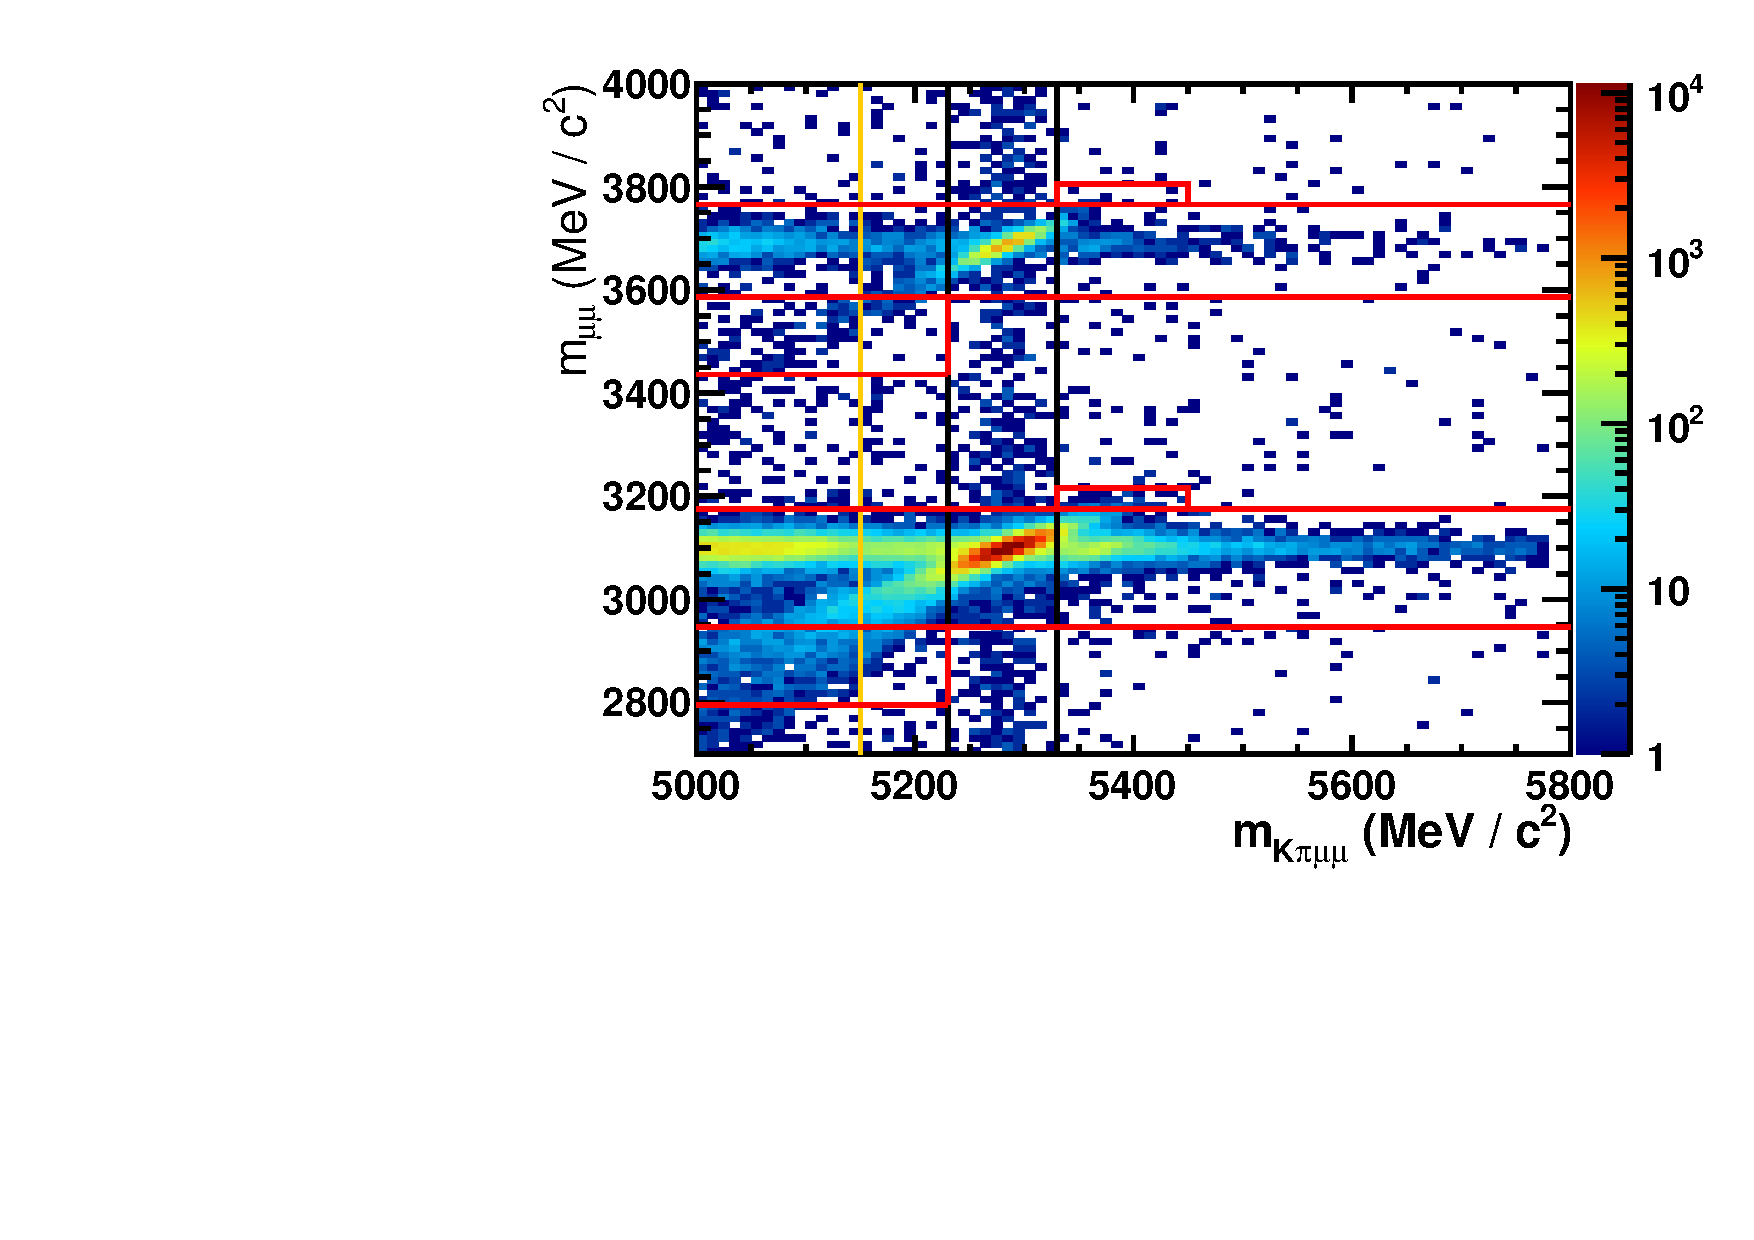
\includegraphics[scale=0.45]{chapter5/figs/sel/c_bm_jpsim_data.pdf}
\caption[ The $K\Ppi\mumu$ versus \mumu invariant mass distribution of \BdToKstmm candidates.   ]
{The $K\Ppi\mumu$ versus \mumu invariant mass distribution of \BdToKstmm candidates.
The charmonium veto regions are indicated by the red lines. 
The yellow line indicates the extent of the lower mass sideband used for the angular analysis.
 \label{fig:selection:jpsiwindows}}
\end{figure}
It is possible to see both the charmonium resonances along with the \BdToKstmm events in the \Bd mass window.
The large low invariant mass tail from radiative and mis-reconstructed \jpsi and \psitwos decays is also evident.

\subsubsection{MVA selection}

In order to select a clean sample of good quality \BdToKstmm candidate decays, a BDT was
%multi-variate analysis (MVA) was
used to take advantage of correlations between the  kinematic, particle identification and topological properties of the candidates.
%The MVA used for this analysis is a Boosted Decision Tree (BDT)~\cite{Breiman,Roe,AdaBoost}. 
The BDT was trained using \BdToJpsiKstar events as signal and upper mass sideband \BdToKstmm events, i.e. events above 5400\mevcc, that pass the pre-selection as background.
The events used for training were selected from an independent data sample taken at \lhcb at \sqs=7\tev in 2010.
Half these events were used for training and half were used to test the performance of the BDT.

The BDT makes use of the following information:
The properties of the \Bd are the \Bd pointing to the primary vertex, the \Bd flight-distance and 
the \Bd impact parameter $\chi^{2}$ with respect to the primary vertex, the \Bd \pt and it's vertex quality ($\chi^{2}$) ;
The properties of the \Kstarz and the di-muon pair are the flight-distance and the impact parameter $\chi^{2}$ 
with respect to the primary vertex (associated to the \Bd), the \Kstar and di-muon \pt and it's vertex quality ($\chi^{2}$);
For each of the final state particles, the impact parameter $\chi^{2}$, the \dllkpi and \dllmu were used.
The value of the BDT output was chosen to optimise the sensitivity to \AFB.


